\section{Deployment és futtatási környezet}

A WatchDB futtatása két fő környezetre bontható: lokális fejlesztői környezetre és éles, felhasználók számára elérhető környezetre. A projekt Next.js alapokra épül, ezért az oldalak, a szerveroldali komponensek és az API route-ok ugyanabban az alkalmazásban találhatók (monorepo-szerű felépítés). Ez egyszerűsíti a deployment folyamatot, mert nincs külön frontend és backend alkalmazás, amelyet eltérő módon kellene telepíteni.

A lokális fejlesztés során a projekt a \texttt{package.json} fájlban megadott parancsokra támaszkodik:

\begin{itemize}
    \item \texttt{npm run dev}: fejlesztői szerver indítása Turbopack használatával;
    \item \texttt{npm run build}: production build elkészítése;
    \item \texttt{npm run start}: az elkészült production build lokális indítása;
    \item \texttt{npm run lint}: statikus kódelemzés futtatása.
\end{itemize}

\begin{figure}[H]
    \centering
    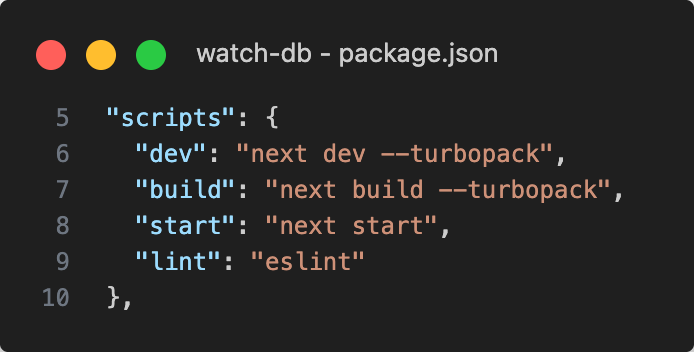
\includegraphics[width=0.85\textwidth]{chapters/chapter-5-systemSpecs/scripts.png}
    \caption{A projekt futtatási scriptjei a \texttt{package.json} alapján}
    \label{fig:watchdb-scripts}
\end{figure}

Az éles környezet szempontjából az alkalmazás Vercel jellegű hostingra illeszkedik. A build folyamat során a szolgáltató telepíti a függőségeket, lefuttatja a production buildet, majd az elkészült alkalmazást elérhetővé teszi a felhasználók számára. A fejlesztési folyamatban ez összekapcsolható a CI/CD szemlélettel: Pull Request esetén preview deployment készülhet, a fő ágra kerülő változtatásból pedig production deployment jöhet létre.

A fejlesztői környezet megfelelő működéséhez a következő konfigurációkra van szükség:

\begin{itemize}
    \item Node.js és npm alapú futtatási környezet;
    \item a Supabase projekthez tartozó publikus URL és anon kulcs;
    \item a TMDB API szerveroldali hozzáférési tokenje;
    \item modern, JavaScript futtatását támogató böngésző;
    \item stabil internetkapcsolat a Supabase, a TMDB API és a TMDB képkiszolgáló eléréséhez.
\end{itemize}

A \texttt{next.config.ts} külön engedélyezi a \texttt{image.tmdb.org} tartományról érkező képek használatát. Erre azért van szükség, mert a filmposzterek és háttérképek nem az alkalmazás saját tárhelyéről, hanem a TMDB képkiszolgálójáról töltődnek be. Az alkalmazás működéséhez ezért nemcsak a saját hosting környezet, hanem a külső képszolgáltató elérhetősége is szükséges.

Fontos döntés, hogy a TMDB hozzáférési token nem kerül kliensoldalra. A filmadatok lekérése a szerveroldali szolgáltatásrétegen keresztül történik, így a böngésző csak az alkalmazás saját API route-jaival kommunikál. Ez a megoldás egyszerűbbé teszi a kulcsok kezelését, és csökkenti annak kockázatát, hogy külső szolgáltatáshoz tartozó érzékeny konfigurációs adat kiszivárogjon.
